%%
%% Author: dariochinelli
%% 2021-04-21
%%

\section{Potenziale nucleare}
Studiamo il potenziale nucleare considerando il nucleo del \emph{deuterio}, chiamato \emph{deutone}, composto da un protone ed un neutrone.

\paragraph{La Cromodinamica Quantistica (QCD)} è una teoria quantistica di campo e relativistica, è una teoria fondamentale che spiega l'interazione tra particelle elementari.
I nucleoni, i componenti del nucleo, protone e neutrone, sono a loro volta composti da \emph{quark}, i quali sono particelle elementari prive di dimensione e con carica frazionaria
\begin{itemize}
\item quark up $u$ ha carica $+\frac{2}{3}$
\item quark down $d$ ha carica $-\frac{1}{3}$
\end{itemize}
i nucleoni sono composti da 3 quark ciascuno e seguono la regola per cui
\begin{itemize}
\item il \textbf{protone} è composto da due quark \emph{up} ed un quark \emph{down}, ha quindi carica totale unitaria:
$$u+u+d = +\frac{2}{3} +\frac{2}{3} -\frac{1}{3} = 1$$
\item il \textbf{neutrone} è composto da due quark \emph{down} ed un quark \emph{up}, ha quindi carica totale nulla:
$$d+d+u = -\frac{1}{3} -\frac{1}{3} +\frac{2}{3} = 0$$
\end{itemize}
\begin{figure}[h]
\centering
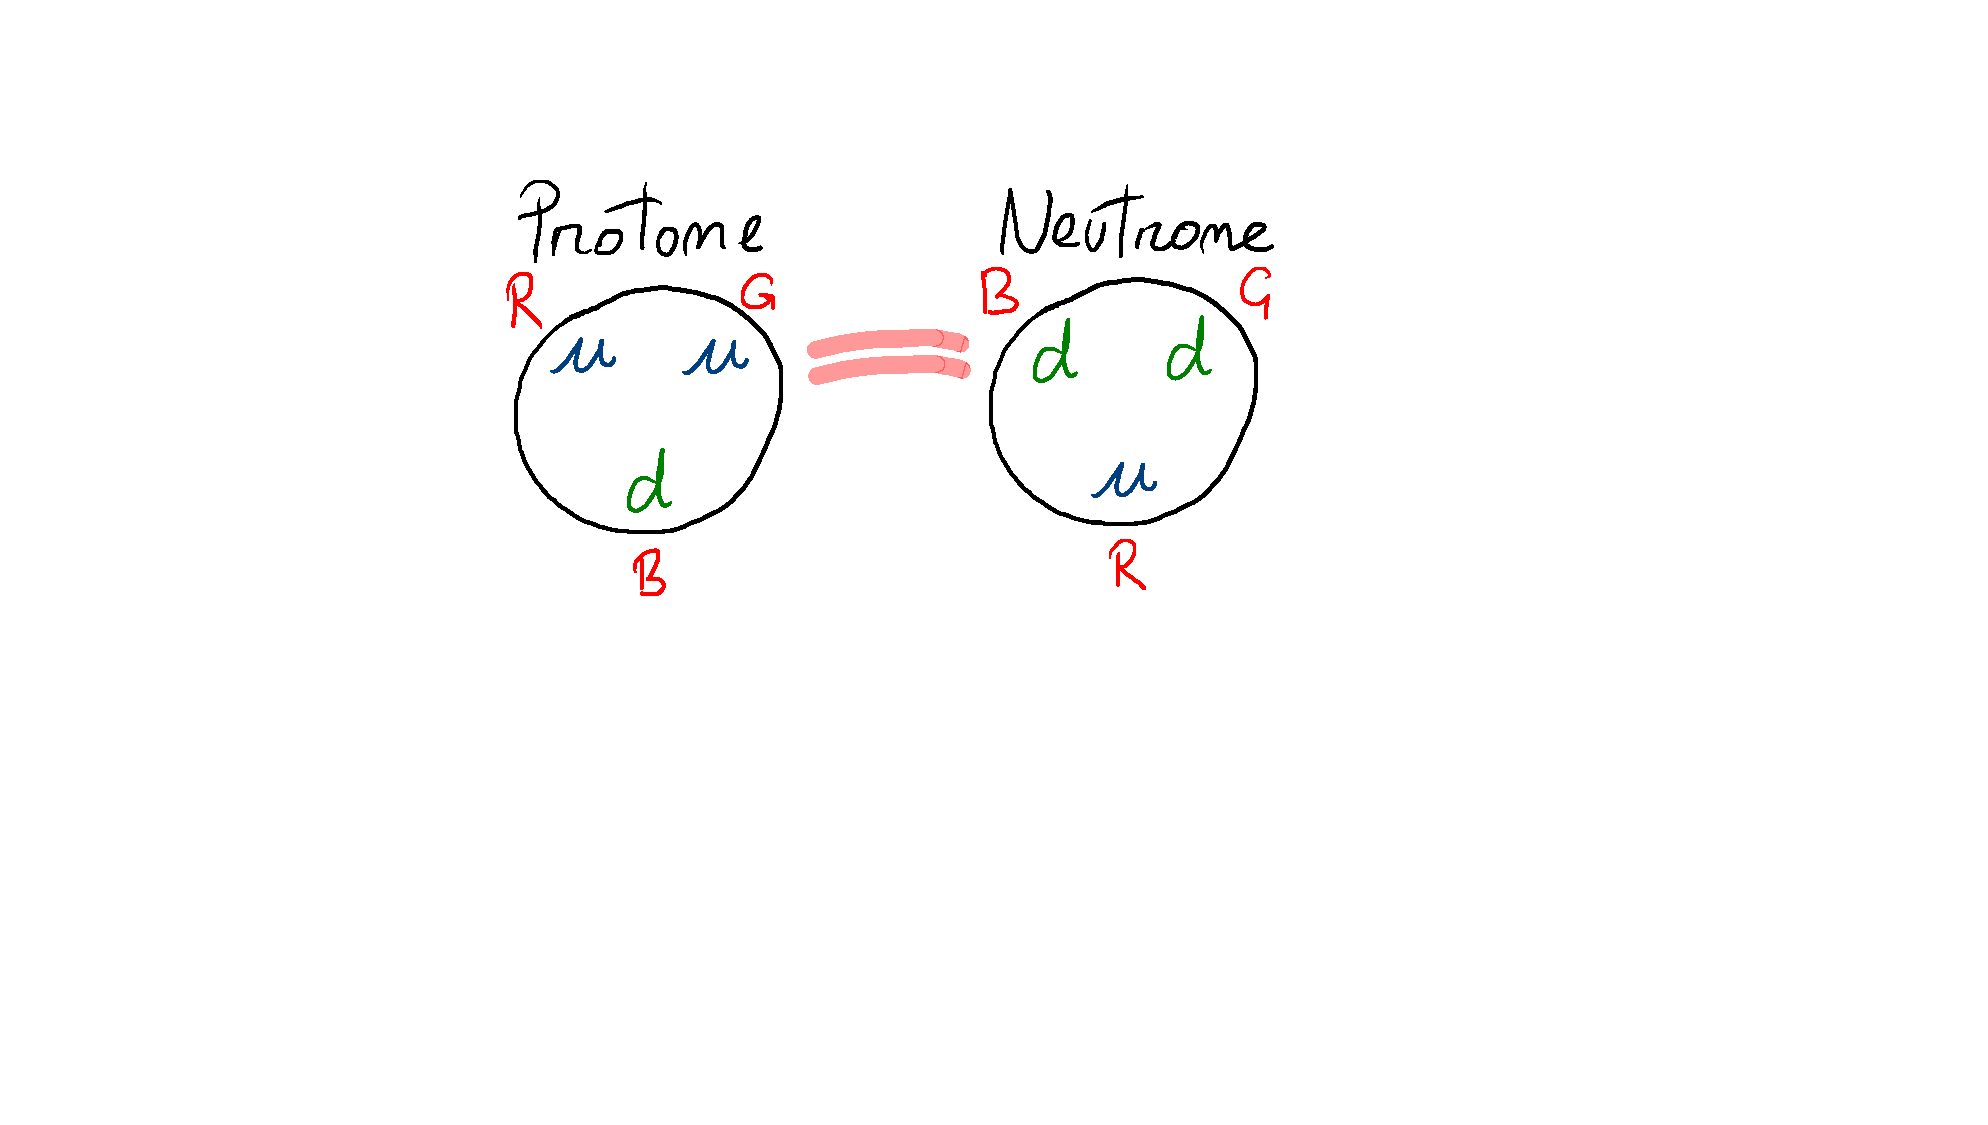
\includegraphics[scale=0.5]{/protone_neutrone_quark}
\caption{CAPTION}
\end{figure}

\paragraph{Carica di colore} I quark hanno anche un secondo tipo di carica: la \emph{carica di colore} che regola l'\emph{interazione forte} tra i quark.
La carica di colore può essere di tre tipi: Red (R), Green (G), Blue (B).
La somma delle tre cariche di colore dei rispettivi quark di un nucleone è nulla
\begin{equation}
R + G + B = 0
\end{equation}
un quark rosso (R) attira un quark verde (G) che attira un quark blu (B), mentre i quark dello stesso colore si respingono.
La teoria fondamentale della QCD esprime come l'interazione nucleare si possa interpretare come la carica di colore residua.

\paragraph{Il potenziale tra nucleoni} è un potenziale di interazione del tipo
\begin{figure}[h]
\centering
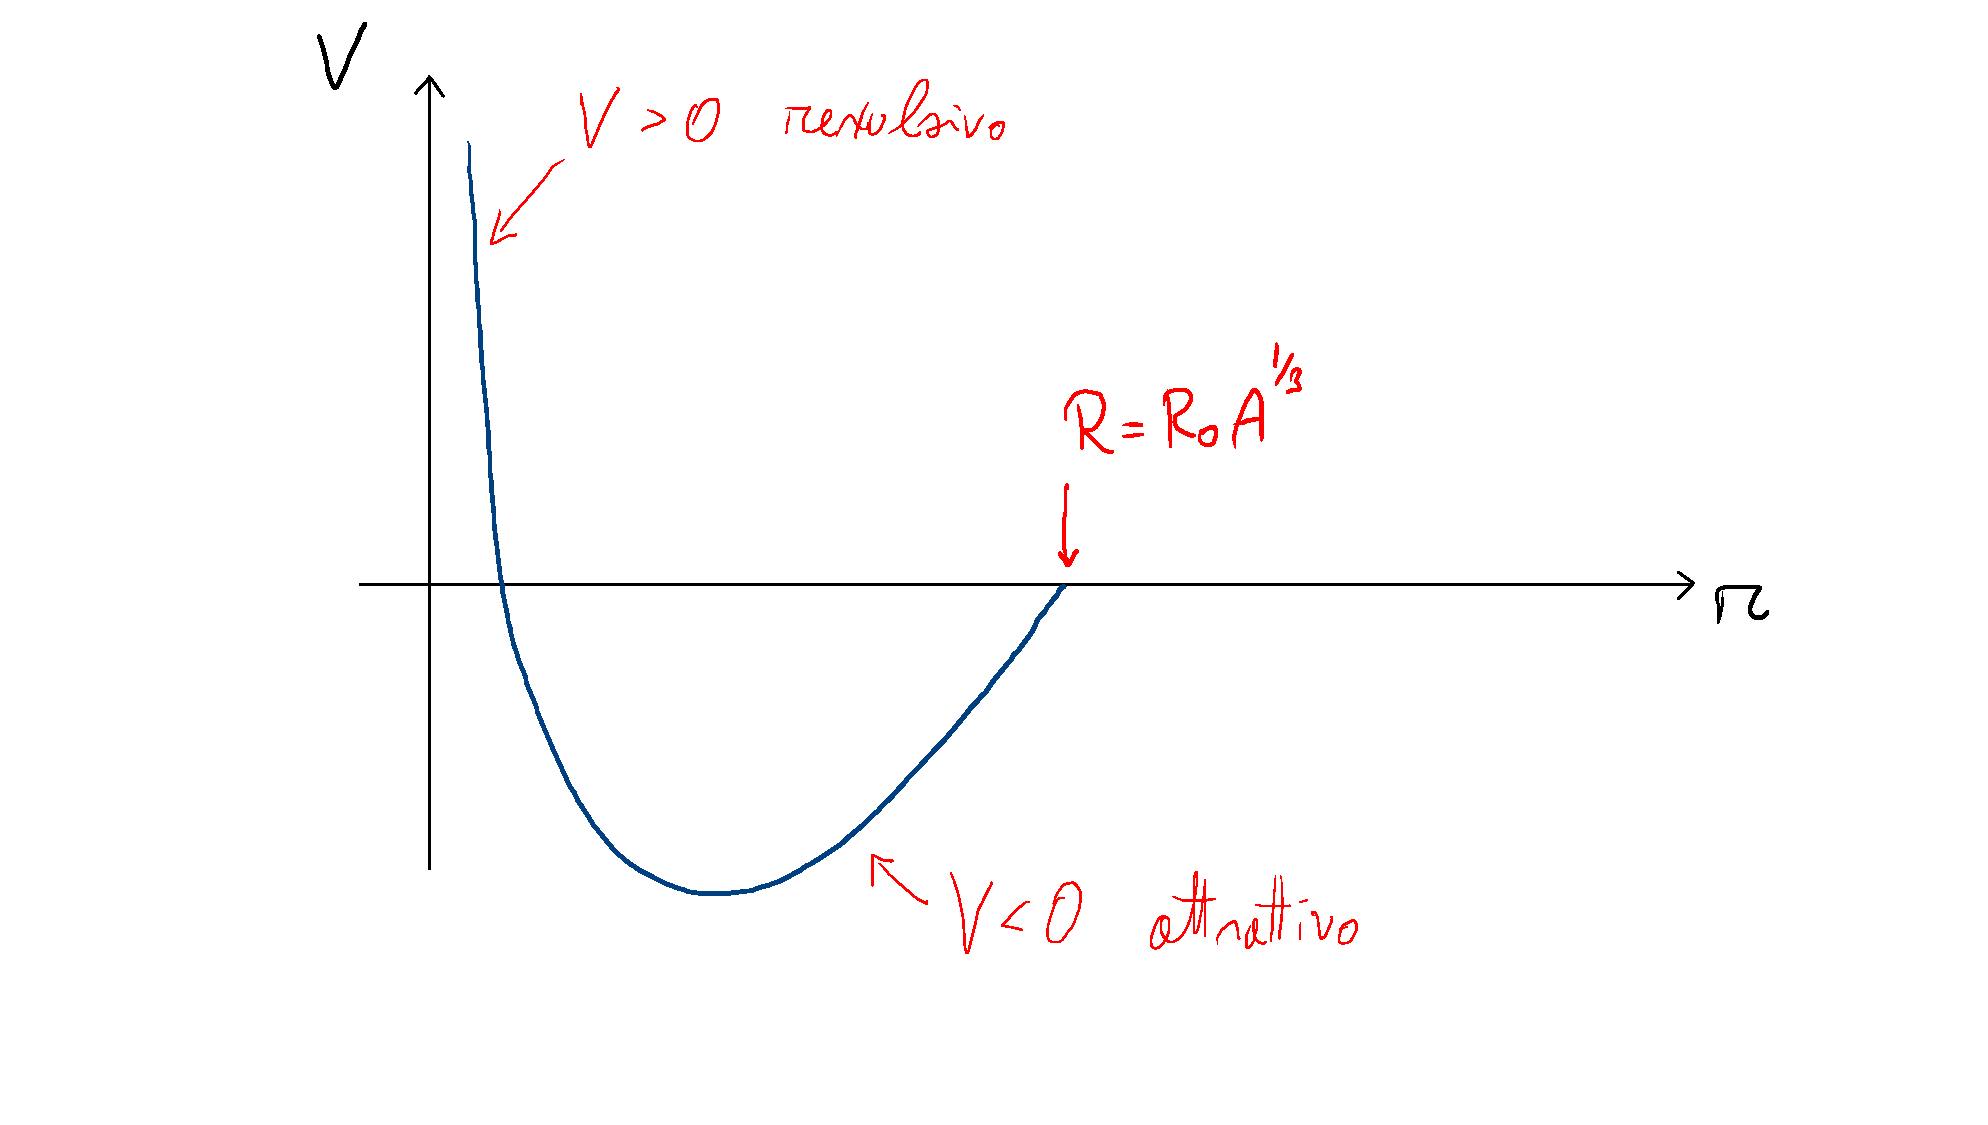
\includegraphics[scale=0.4]{/potenziale_nucleare_1}
\caption{CAPTION}
\end{figure}
Nella prima parte del potenziale si ha che per piccole distanze è \emph{positivo}, ovvero repulsivo, poiché altrimenti i nuclei \underline{privi di dimensione (?)} collasserebbero, ciò è legato al Principio di Esclusione di Pauli, nella seconda parte il potenziale è \emph{attrattivo} ed è ciò che "intrappola" i nucleoni all'interno del nucleo, inoltre oltre alla distanza data da $R = R_0 A^{\frac{1}{3}}$ la forza nucleare è nulla.

\paragraph{Il Deutone} è il nucleo del deuterio, è composto da un protone e un neutrone ed è il più semplice nucleo su cui studiare la forza nucleare.
Del deutone conosciamo l'energia di legame $E_B = \SI{-2.225}{MeV}$ e la distanza tra i nucleoni $R = \SI{2.1}{fm}$ ottenuti sperimentalmente.
Conosciamo inoltre che lo stato legato del deuterio è quello in cui gli spin sono paralleli, dato ottenuto dalla misurazione del momento magnetico, per cui lo spin del deutone è $S = 1$.
\begin{figure}[h]
\centering
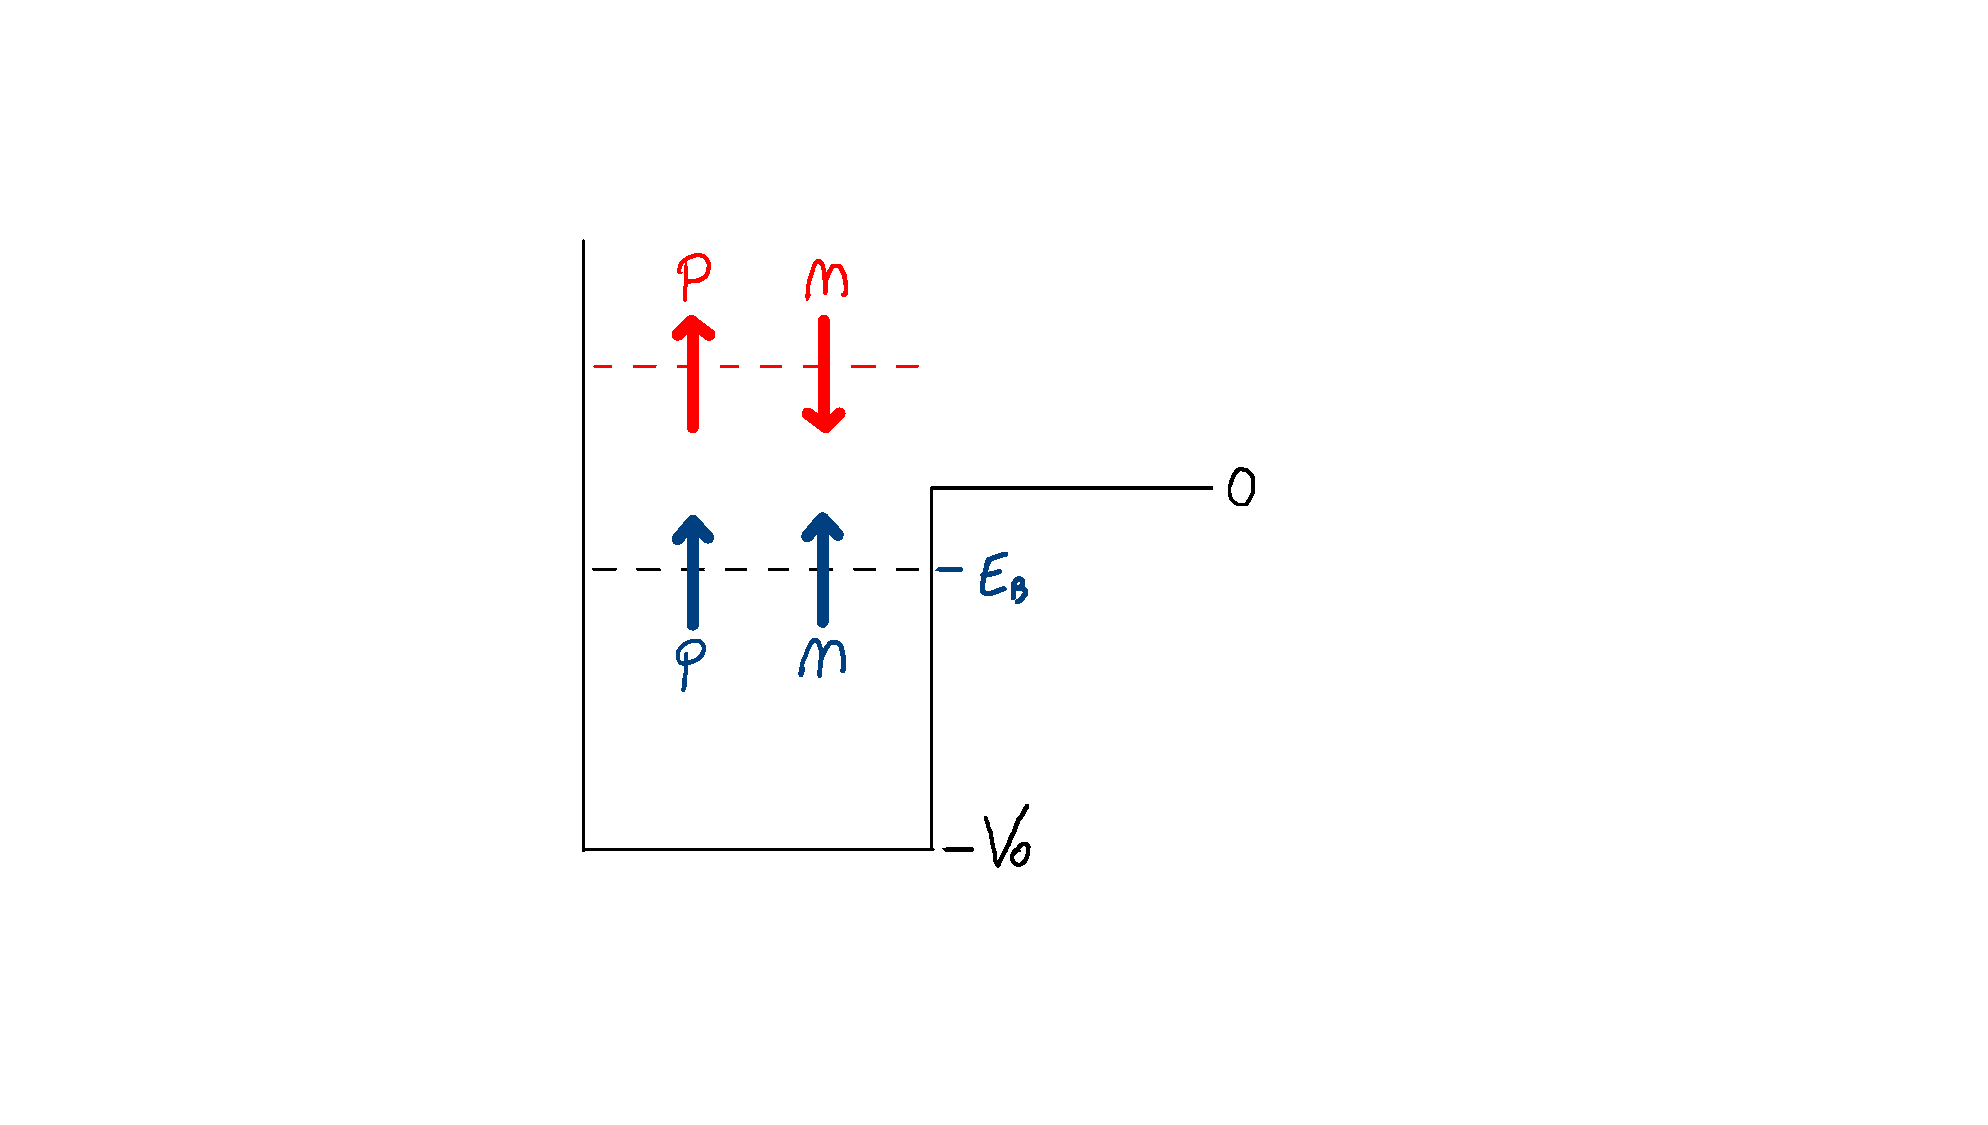
\includegraphics[scale=0.5]{/spin_deutone}
\caption{CAPTION}
\end{figure}
Uno stato con spin anti-parallelo corrisponde ad uno stato non legato, quindi fuori dalla buca di potenziale.
L'interazione nucleare dipende fortemente dallo spin.

Cerco ora il valore della buca di potenziale $V_0$, sommo l'energia cinetica $KE$ con l'energia potenziale $PE$
\begin{equation}
\begin{split}
E & = KE + PE \\
E_B & = KE + V_0
\end{split}
\end{equation}
scrivendo la funzione d'onda trovo il legame con il potenziale $V$
\begin{equation}
\begin{split}
H \psi & = E \psi \\
- \frac{\hbar^2}{2m} \frac{d^2}{dr^2} \psi + V \psi & = E \psi
\end{split}
\end{equation}
Il potenziale di questa buca è
\begin{equation}
V = 
\Bigg\{\begin{array}{l}
V_0 \quad\mbox{zona 1: dentro la buca} \\
0 \quad\mbox{ zona 2: altrove}
\end{array}
\end{equation}
Scrivo l'equazione di Schrodinger nella zona 1, in cui ho $V = V_0$
\begin{equation}
\begin{split}
- \frac{\hbar^2}{2m} \frac{d^2 \psi}{d r^2} + V_0 \psi & = E \psi \\
\frac{d^2 \psi}{d r^2} & = -\frac{2m}{\hbar^2} (E - V_0) \psi \\
\frac{d^2 \psi}{d r^2} & = - K^2 \psi \quad\quad \mbox{con } K^2 = \frac{2m}{\hbar^2} (E - V_0)
\end{split}
\end{equation}
la soluzione ha un andamento oscillatorio ed in generale è
\begin{equation}
\psi(r) = A \sin Kr + B \cos Kr
\end{equation}
calcolo $A$ e $B$ imponendo le condizioni al contorno:
\begin{equation}
\psi (0) = 0 \quad\Rightarrow\quad \psi(0) = A \sin 0 + B \cos 0 = 0 \quad\Rightarrow\quad B=0
\end{equation}
per cui diventa
\begin{equation}
\psi = A \sin K r
\label{psi_1}
\end{equation}
Scrivo l'equazione di Schrodinger nella zona 2, in cui ho $V =0$
\begin{equation}
\begin{split}
\frac{d^2 \psi}{d r^2} & = -\frac{2m}{\hbar^2} E \psi \\
\frac{d^2 \psi}{d r^2} & = L^2 \psi \quad\quad \mbox{con } L^2 = - \frac{2m}{\hbar^2} E
\end{split}
\end{equation}
la soluzione ha un andamento esponenziale ed in generale è
\begin{equation}
\psi(r) = C e^{L r} + D e^{- L r}
\end{equation}
di cui so che deve appartenere allo spazio di Hilbert, per cui la parte $e^{L r}$ non è soluzione in quanto non verifica la condizione $|\psi|^2 < \infty$, per cui diventa
\begin{equation}
\psi(r) = D e^{- L r} 
\label{psi_2}
\end{equation}
Eguagliando le funzioni d'onda \ref{psi_1} e \ref{psi_2} e le loro derivate in corrispondenza della frontiera $r = R$ trovo
\begin{equation}
\Bigg\{\begin{array}{l}
\psi_{1}(R) = \psi_{2}(R)\\
\psi_{1}'(R) = \psi_{2}'(R)
\end{array}
\quad\Rightarrow\quad 
\Bigg\{\begin{array}{l}
A \sin K R = D e^{ - L R }\\
K A \sin K R = -L D e^{ - L R }
\end{array}
\end{equation}
dividendo una con l'altra le equazioni del sistema trovo la relazione seguente in funzione dei parametri $K$ ed $L$
\begin{equation}
\begin{split}
K & = \sqrt{\frac{2m}{\hbar^2} (E - V_0)} \in \mathbb{R} \\
L & = \sqrt{- \frac{2m}{\hbar^2} E} \in \mathbb{R}
\end{split}
\end{equation}
che quindi diventa
\begin{equation}
\begin{split}
& K \cot K R = - L \\
& \sqrt{\frac{2m}{\hbar^2} (E - V_0)} \cot \Bigl[ R \sqrt{\frac{2m}{\hbar^2} (E - V_0)} \Bigr] = - \sqrt{- \frac{2m}{\hbar^2} E}
\end{split}
\end{equation}
da cui, inserendo i dati sperimentali, 
\begin{equation}
\begin{split}
E & = \SI{-2.225}{MeV} \\
R & = \SI{2.1}{fm}
\end{split}
\end{equation}
e la massa corrisponde alla massa ridotta tra il protone ed il neutrone
\begin{equation}
m = \frac{m_n m_p}{m_n + m_p} \simeq \frac{m_p^2}{2 m_p} = \frac{m_p}{2}
\end{equation}
trovo il valore della buca di potenziale
\begin{equation}
V_0 = \SI{-36}{MeV}
\end{equation}
(non è ben noto come sia davvero possibile risolvere l'equazione del tipo $x \cot a x = b$ ma ok, prendiamo atto del risultato precedente e andiamo avanti).

Risulta quindi che la buca di potenziale del Deutone è profonda $\SI{-36}{MeV}$ di cui solo $\SI{-2.225}{MeV}$ sono di energia potenziale, \emph{di legame}, mentre circa $\SI{-34}{MeV}$ sono di energia cinetica.

Per il ferro $^{56}_{26}Fe$ ad esempio si ha un'energia di legame media di circa $\SI{8}{MeV / nucleone}$, mentre
per il deutone $^{2}_{1}He$ si ha circa $\SI{1.1}{MeV / nucleone}$.

Troviamo tre punti notevoli della funzione d'onda:

\begin{itemize}
\item Quanto vale la funzione d'onda nel punto $r=R$?
In tale punto la funzione vale $\sin K R$ per cui conoscendo i dati trovo
\begin{equation}
\begin{split}
& R = \SI{2.1}{fm} \\
& K = \sqrt{ \frac{2m}{\hbar^2} (E - V_0) } \simeq \SI{0.9}{fm^{-1}} \\
& \sin K R = \sin (0.9 \cdot 2.1) = 0.95
\end{split}
\end{equation}

\item In che punto si ha il valore massimo della funzione d'onda?
\begin{equation}
\begin{split}
& \sin K r = 1 \\
& K r = \frac{\pi}{2} \\
& r = \frac{\pi}{2} \frac{1}{K} \simeq \SI{1.74}{fm}
\end{split}
\end{equation}

\item In che punto la funzione d'onda vale circa $\frac{1}{3}$?
\begin{equation}
\begin{split}
e^{ - L r } & \quad L = \sqrt{\frac{2mE}{\hbar^2}} \to \frac{1}{L} = \SI{4.4}{fm} \\
e^{ - L r } & \rightarrow e^{ \frac{-L}{L}} = e^{ -1 } = 0.37
\end{split}
\end{equation}
\end{itemize}
La funzione d'onda si estende di fuori della buca di potenziale, a distanze oltre i $\SI{5}{fm}$, questo perché il deutone è uno stato poco legato.
Nel caso della molecola di idrogeno l'atomo è molto ben localizzato all'interno della buca di potenziale.

\subsection{Collisione neutrone protone}
Studiamo ora il potenziale nucleare partendo dalla collisione tra protone e neutrone.
\paragraph{La produzione di un fascio di neutroni} la collisione di un fascio di protoni contro un bersaglio si ottengono molteplici particelle, applicando un potenziale elettrico dopo il target si "selezionano" quelle cariche e quelle neutre, che continueranno inalterate nel loro moto, come i neutroni ed i pioni neutri o $\pi_0$.
Con una buona definizione temporale posso anche discriminare i neutroni in base all'energia, i primi saranno i più energetici.

Il potenziale di interazione tra un neutrone ed un target sarà del tipo visto nei paragrafi precedenti, quindi una buca di potenziale finita.
I neutroni incidenti sono liberi, per cui avranno energia maggiore rispetto allo zero della buca di potenziale.
\begin{figure}[h]
\centering
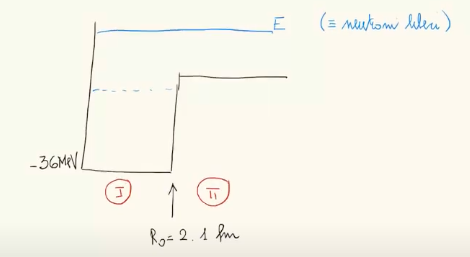
\includegraphics[scale=0.7]{/potenziale_neutroni_liberi}
\caption{CAPTION}
\end{figure}
L'equazione che descrive il neutrone è
\begin{equation}
\begin{split}
-\frac{\hbar^2}{2m} \frac{d^2 \psi}{dr^2} + V \psi & = E \psi \\
\mbox{zona 1} \quad\quad  & \frac{d^2 \psi}{dr^2} = - \frac{2m}{\hbar^2} (E-V_0) \psi \\
\mbox{zona 2} \quad\quad  & \frac{d^2 \psi}{dr^2} = - \frac{2m}{\hbar^2} \psi
\end{split}
\end{equation}
noto ora che il termine $ k^2 = \frac{2m}{\hbar^2} (E-V_0)$ è positivo ed anche il termine $L^2 = \frac{2m}{\hbar^2}$ è positivo.
In entrambe le zone si ha quindi un andamento oscillatorio della funzione d'onda
\begin{equation}
\begin{split}
\mbox{zona 1} \quad\quad  & \psi = A \sin k r + B \cos k r = A \sin k r \\
\mbox{zona 2} \quad\quad  & \psi = C \sin k r + D \cos k r = E \sin ( L r + \delta )
\end{split}
\end{equation}
applicando le condizioni al bordo e di continuità trovo
\begin{equation}
\begin{split}
& A \sin k r_0 = E \sin (L r_0 + \delta) \\
& k A \cos k r_0 = L E \cos (L r_0 + \delta) \\
\Rightarrow\quad & k \cot k r_0 = L \cot (L r_0 + \delta)
\end{split}
\end{equation}
dove ricordando i valori di 
\begin{equation}
\begin{split}
& k = \sqrt{\frac{2m}{\hbar^2}(E-V_0)} \\
& L = \sqrt{\frac{2m}{\hbar^2}E} \\
& r_0 = \SI{2.1}{fm}
\end{split}
\end{equation}
vedo che il solo termine da ricavare rimane $\delta$.

La sezione d'urto differenziale e totale sono
\begin{equation}
\begin{split}
& \frac{d\sigma}{d\Omega} = \frac{1}{k^2} \sin \delta \\
& \sigma_{tot} = \frac{4\pi}{k^2} \sin^2 \delta
\end{split}
\end{equation}
da queste espressioni teoriche si ricava
\begin{equation}
\sigma_{teorico} = \SI{5}{barn} \quad\quad \SI{1}{barn} = \SI{e-28}{m^2}
\end{equation}
e dall'esperimento si ricava
\begin{equation}
\sigma_{sperimentale} = \SI{20}{barn}
\end{equation}
sussiste quindi una grossa discrepanza tra i due valori. 

Il potenziale visto sopra è un potenziale attrattivo ed è quello che permette di avere uno stato legato con spin parallelo con $S=1$, stato di tripletto in cui compaiono tre contributi $1 \hbar, 0, -1 \hbar$, mentre $S=0$ si ha solo nel caso con spin antiparalleli.

La sezione d'urto totale è data dalla seguente relazione, nella trattazione precedente abbiamo considerato solo il primo termine
\begin{equation}
\begin{split}
\sigma_{tot} & = \frac{3}{4} (\delta_{S=1}) + \frac{1}{4} (\delta_{S=0}) \\
20 & = 0.75 \cdot 5 + 0.25 \cdot \sigma_{S=0} \\
\sigma_{S=0} & = \SI{65}{barn}
\end{split}
\end{equation}
da cui abbiamo ricavato dal punto di vista sperimentale che l'interazione nucleare ha una forte dipendenza dallo spin relativo alle due particelle.
Quindi non si può trascurare lo spin nella trattazione di questa interazione.

\subsection{ultima parte}
Mettendo su un grafico la $\delta$ in funzione dell'energia $E$, trovo due curve che rappresentano la dipendenza per $S = 1$ e per $S = 0$, si osserva che per una determinata energia entrambi gli andamenti cambiano di segno, tale energia è pari a $\SI{300}{MeV}$
\begin{figure}[h]
\centering
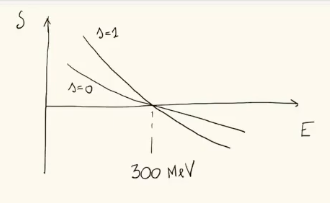
\includegraphics[scale=0.7]{/fase_energia_potnucl}
\caption{CAPTION}
\label{delta_energ}
\end{figure}
\begin{equation}
\delta_{tot} = \frac{4\pi}{k^2} \sin^2 \delta
\end{equation}

Studiando i parametri in funzione del potenziale $V_0$ osservo che, 
\begin{equation}
V_0 < 0 
\quad\Rightarrow\quad 
k > L \quad\Rightarrow\quad 
\lambda_k < \lambda_L \quad \mbox{dove } k = \frac{2\pi}{\lambda}
\end{equation}
dati
\begin{equation}
k = \sqrt{\frac{2m}{\hbar^2}(E-V_0)} \quad\quad L = \sqrt{\frac{2m}{\hbar^2}E}
\end{equation}
graficando la funzione d'onda $\psi$ in funzione della distanza $r$ vedo che le due zone devono essere unificate imponendo l'uguaglianza e che il parametro $\delta$ permette ciò.
\begin{figure}[h]
\centering
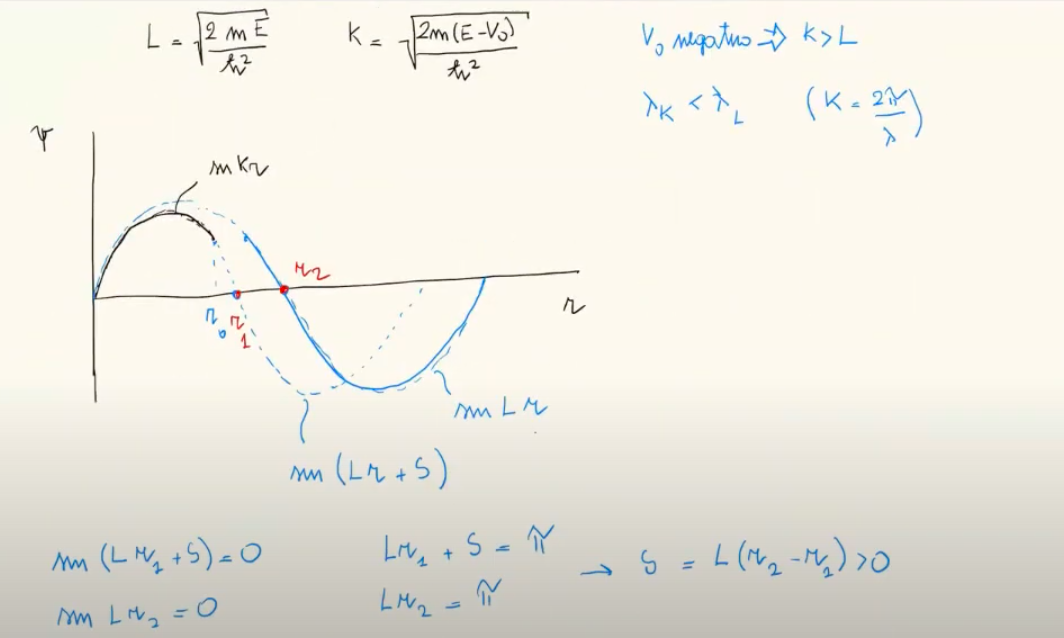
\includegraphics[scale=0.1]{/funzione_donda_potenziale}
\caption{CAPTION}
\end{figure}
In particolare presi due punti $r_1$ ed $r_2$ intersezioni tra il grafico e l'asse delle ascisse, cioè dove la funzione si annulla, trovo le relazioni
\begin{equation}
\begin{split}
 & \sin (L r_1 + \delta) = 0 \quad\Leftrightarrow\quad L r_1 + \delta = \pi \\
 & \sin (L r_2) = 0 \quad\Leftrightarrow\quad L r_2 = \pi
\end{split}
\end{equation}
da cui
\begin{equation}
\delta = L (r_2 - r_1) > 0
\end{equation}

Supponiamo che il potenziale abbia un andamento del tipo 
\begin{figure}[h]
\centering
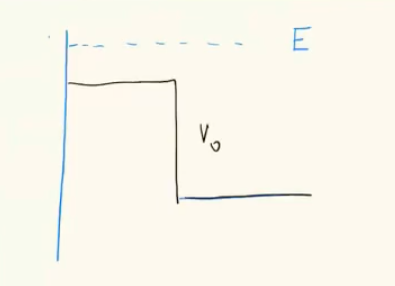
\includegraphics[scale=0.7]{/potenziale_due}
\caption{CAPTION}
\end{figure}
la descrizione matematica sarà equivalente alle precedenti, e si ottiene
\begin{equation}
\begin{split}
\psi_1 = A \sin k r \\
\psi_2 = E \sin (Lr + \delta)
\end{split}
\end{equation}
ma in questo caso il potenziale è positivo $V_0 > 0$ per cui
\begin{equation}
L > k \quad\Rightarrow\quad \lambda_L < \lambda_k
\end{equation}
cercando dove le funzioni si annullano trovo
\begin{equation}
\begin{split}
\sin L r_1 & = 0 \quad\Leftrightarrow\quad L r_1 = \pi \\
\sin L r_2 & = 0 \quad\Leftrightarrow\quad L r_2 + \delta = \pi 
\end{split}
\end{equation}
da cui
\begin{equation}
\delta = L (r_1 - r_2) < 0
\end{equation}
tornando al grafico \ref{delta_energ} vedo che a basse energie $(E< \SI{300}{MeV})$, per cui delta è maggiore di zero, si ha un potenziale attrattivo, mentre ad energie maggiori, per cui delta è negativo, si ha un potenziale repulsivo.

Possiamo allora caratterizzare completamente il potenziale nucleare,
\begin{equation}
r_{\alpha} \sim \SI{0.5}{fm} 
\quad
R_{0} \sim \SI{2.1}{fm}
\end{equation}
per cui tra $0$ e $r_{\alpha}$ il potenziale è positivo (repulsivo) e tra $r_{\alpha}$ ed $R_0$ è negativo (attrattivo).
All'interno del nucleo le particelle si dispongono in modo ordinato e non si comprimono, la densità in funzione del numero atomico è costante, è satura.
Quindi aumentando il numero di massa aumenta il volume del nucleo, poiché la densità è costante.
\emph{Il volume di un nucleo è direttamente legato al numero di nucleoni.}










